\documentclass{beamer}
\usepackage{lmodern} % Add the lmodern package to fix missing font shapes
\usepackage{beamerthemeDHBW} % Include the package
\usepackage[overlay, absolute]{textpos}
\usepackage{bookmark}
\usepackage{pgfplots}
\usepackage{tikz}
\usepackage{amssymb} % Add the amssymb package to fix missing font shape
\usepackage{listings}
\newcommand{\internetadresse}{https://www.dhbw-stuttgart.de}
\pgfplotsset{compat=1.18}

\lstset{
    basicstyle=\ttfamily\scriptsize,
    keywordstyle=\color{blue},
    commentstyle=\color{green!60!black},
    numbers=left,
    numberstyle=\tiny\color{gray},
    frame=single,
    backgroundcolor=\color{lightgray},
    showspaces=false,
    showstringspaces=false,
    showtabs=false,
    breaklines=true,
    tabsize=4
}


%Information to be included in the title page:
\title{Java-TX Compiler in Java-TX}
\author{Julian Schmidt}
\institute{DHBW Stuttgart}
\date{2024}

\usetheme{DHBW}

\begin{document}

\maketitle

\begin{frame}
    \frametitle{Agenda}
    \begin{enumerate}
        \item Motivation
        \item Aufbau der Umgebung
        \item Bugs/Probleme
              \begin{enumerate}
                  \item Überschreiben von Methoden
                  \item Kompatibilität mit funktionalen Interfaces
              \end{enumerate}
        \vspace*{-\baselineskip}
        \item Fazit

    \end{enumerate}
\end{frame}

\begin{frame}
    \frametitle{Motivation I}

    \begin{itemize}
        \item Welche Features fehlen noch in Java-TX?
        \item Welche Bugs gibt es?
        \item Wie performant is Java-TX für größere Projekte?
        \item Vorteile/Nachteile zu Java in der Praxis
    \end{itemize}

\end{frame}

\begin{frame}
    \frametitle{Motivation II}
    \begin{center}
        \begin{tikzpicture}[scale=3]
            \draw (1,0) -- (0,0) -- (0,1) -- (3,1) -- (3,0) -- (2,0) -- (2, -1.1) -- (1, -1.1) -- cycle;
            \node at (0.5, 0.5) {JTX};
            \node at (1.5, -0.55) {JTX};
            \node at (2.5, 0.5) {BC};
            \draw (3.1,-1.1) -- (2.1,-1.1) -- (2.1,-0.1) -- (5.1,-0.1) -- (5.1,-1.1) -- (4.1,-1.1) -- (4.1, -2.2) -- (3.1, -2.2) -- cycle;
            \node at (2.6, -0.6) {JTX};
            \node at (3.6, -1.6) {JAVA};
            \node at (4.6, -0.6) {BC};
        \end{tikzpicture}
    \end{center}
\end{frame}

\begin{frame}[fragile]{Vergleich Sourcecode}
    \begin{columns}
        \begin{onlyenv}<1->
        \begin{column}{0.5\textwidth}
            \begin{lstlisting}[language=java]
public class FunNClass extends ClassOrInterface {
  private static GenericDeclarationList createGenerics(List<GenericRefType> funNParams) {
    var generics = new ArrayList<GenericTypeVar>();
    for (GenericRefType param : funNParams) {
      generics.add(...);
    }
    return new GenericDeclarationList(generics, new NullToken());
  }
}
            \end{lstlisting}
        \end{column}
        \end{onlyenv}
        \begin{onlyenv}<1> 
        \begin{column}{0.5\textwidth}
            \begin{lstlisting}[language=java]
public class FunNClass extends ClassOrInterface {
  private static createGenerics(funNParams) {


    var generics = new ArrayList<GenericTypeVar>();
    for (GenericRefType param : funNParams) {
        generics.add(...);
    }
    return new GenericDeclarationList(generics, new NullToken());
  }
}
            \end{lstlisting}
        \end{column}

        \end{onlyenv}
        \begin{onlyenv}<2->
        \begin{column}{0.5\textwidth}
            \begin{lstlisting}[language=java, escapechar=!]
public class FunNClass extends ClassOrInterface {
  private static GenericDeclarationList createGenerics(Iterable<? extends GenericRefType> var0) {
    List var1 = null;
    var1 = (List)(new ArrayList());
    Iterator var10000 = var0.iterator();
    while(var10000.hasNext()) {
      GenericRefType var2 = (GenericRefType)var10000.next();
      var1.add(...);
    }
    return new GenericDeclarationList(var1, new NullToken());
  }
}
            \end{lstlisting}
        \end{column}
        \end{onlyenv}
    \end{columns}
\end{frame}

\begin{frame}{Aufbau der Umgebung I}
        \begin{enumerate}
        \item Compiler soll sukzessive in Java-TX umgeschrieben werden
        \item Umgebung mit .java und .jav Dateien
        \item Ziel: Auf JVM ausführbare .class Dateien
        \item Java-TX Compiler kann .java Dateien lesen \\
        \(\rightarrow\) Abhängigkeiten zu Java Dateien möglich
        \item Java-TX Compiler muss vor javac aufgerufen werden
    \end{enumerate}
\end{frame}

\begin{frame}[fragile]
    \frametitle{Aufbau der Umgebung II - make}
    Erster Ansatz mit make:
    \begin{lstlisting}
    # Use find to locate all .java and .jav files recursively
    JAVASOURCES := $(shell find $(SRCDIR) -name '*.java')
    JAVSOURCES := $(shell find $(SRCDIR) -name '*.jav')

    # Convert .java/.jav files to .class files with the same directory structure
    JAVACLASSES := $(patsubst $(SRCDIR)/%.java,$(DESTDIR)/%.class,$(JAVASOURCES))
    JAVCLASSES := $(patsubst $(SRCDIR)/%.jav,$(DESTDIR)/%.class,$(JAVSOURCES))

    # Rule for compiling .jav files
    $(DESTDIR)/%.class: $(SRCDIR)/%.jav
    java -jar $(JTX) -d "$(dir $@)" -cp "$(SRCDIR):$(DESTDIR):target/dependencies/" $<
    # Rule for compiling .java files
    $(DESTDIR)/%.class: $(SRCDIR)/%.java
	$(JC) -nowarn -d $(DESTDIR) -cp "$(SRCDIR):$(DESTDIR):target/dependencies/*" $(JFLAGS) $<
\end{lstlisting}
\end{frame}


\begin{frame}[fragile]{Aufbau der Umgebung III}
    Probleme:
    \begin{enumerate}
        \item javac compiliert und trackt Änderungen der Abhängigkeiten automatisch
        \item javac ist sehr langsam wenn für jede Datei einzeln aufgerufen (viele mehrfache Compilierungen)
    \end{enumerate}
    \begin{columns}
        \begin{column}{0.5\textwidth}
            \begin{lstlisting}
javac src/main/java/de/dhbwstuttgart/typedeployment/TypeInsert.java
javac src/main/java/de/dhbwstuttgart/typedeployment/TypeInsertPlacer.java
...
javac src/main/java/Main.java
                \end{lstlisting}
            $\sim{}$5min Compilerzeit
        \end{column}
        \begin{column}{0.5\textwidth}
            \begin{lstlisting}
javac src/main/java/de/dhbwstuttgart/typedeployment/TypeInsert.java src/main/java/de/dhbwstuttgart/typedeployment/TypeInsertPlacer.java ... src/main/java/Main.java
                \end{lstlisting}
            $\sim{}$2sec Compilerzeit
        \end{column}
    \end{columns}
\end{frame}

\begin{frame}[fragile]{Aufbau der Umgebung IV - compile script}
    Gegeben: Quellverzeichnis, Zielverzeichnis
    \begin{enumerate}
        \item Suche rekursiv alle .java und .jav Dateien im Quellverzeichnis und speichere sie jeweils in einer Liste
        \item Überprüfe für jede Quelldatei, ob die zugehörige .class Datei im Zielverzeichnis existiert und ob die Zieldatei neuer als die Quelldatei ist
              \begin{itemize}
                  \item Wenn ja, gehe weiter zur nächsten Datei
                  \item Wenn nein, füge die Quelldatei zur Liste der zu kompilierenden Dateien hinzu
              \end{itemize}
\vspace*{-\baselineskip}
        \item Rufe den Java-TX Compiler mit allen Dateien in der jav-Liste als Argumente auf
              \lstinline{java -jar $JAVATX_COMPILER_PATH -d $DESTDIR -cp "$SRCDIR:$DESTDIR:target/dependencies/" "${JAV_CHANGED[@]}"}
        \item Rufe den javac Compiler mit allen Dateien in der java-Liste als Argumente auf
              \lstinline{javac -d $DESTDIR -cp "$SRCDIR:$DESTDIR:target/dependencies/*" $JAVAC_FLAGS "${JAVA_CHANGED[@]}"}
    \end{enumerate}

\end{frame}

\begin{frame}[fragile]{Bugübersicht}
    \begin{center}
        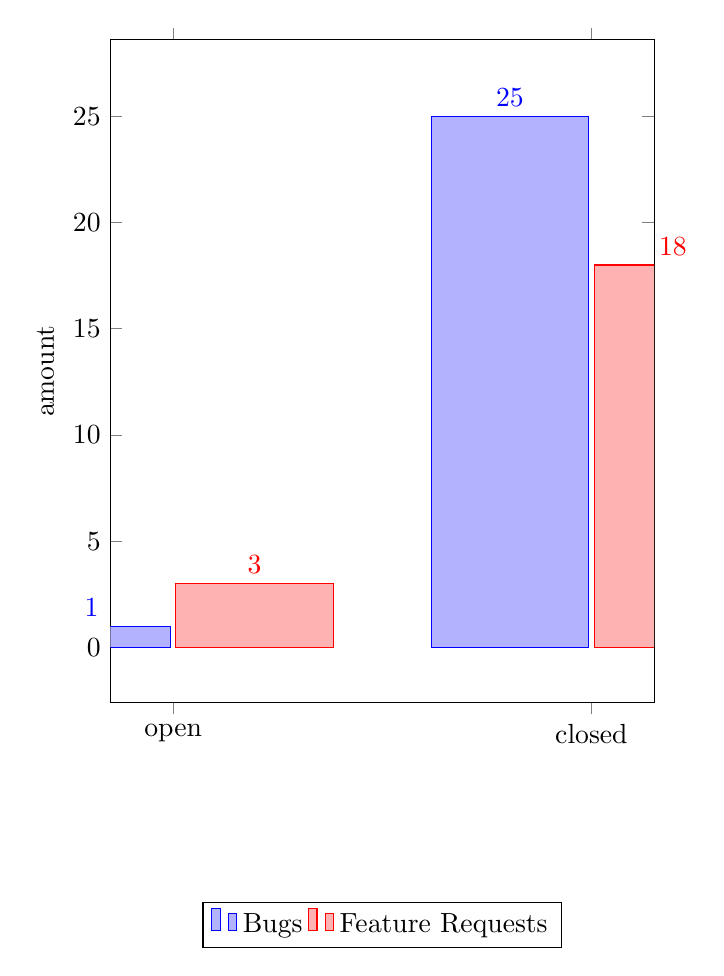
\begin{tikzpicture} \begin{axis}[ ybar, enlargelimits=0.15, legend style={at={(0.
                                5,-0.3)}, anchor=north,legend columns=-1}, ylabel={amount}, symbolic x
                coords={open,closed}, xtick=data, nodes near coords, nodes near coords
                align={vertical}, width=0.7\textwidth, height=10cm, bar width=2cm] 
                \addplot coordinates {(open,1) (closed,25) };
                \addplot coordinates {(open,3) (closed,18) };
                \legend{Bugs,Feature Requests}
            \end{axis} 
        \end{tikzpicture}
    \end{center}
\end{frame}

\begin{frame}[fragile]{Primitive Typen in Java-TX}
    \begin{itemize}
        \item Java erlaubt neben Referenztypen auch primitive Datentypen (int, boolean, ...)
        \item Java-TX erlaubt primitive Datentypen zwar im Quellcode, wandelt diese aber in die korrespondierende Wrapperklasse um (Integer, Boolean, ...)
    \end{itemize}

    \begin{columns}
        \begin{column}{0.5\textwidth}
            \begin{lstlisting}[language=java]
int a = 10; 
boolean b = true;
float c = 10.0f;
            \end{lstlisting}
        \end{column}
        \begin{column}{0.5\textwidth}
            \begin{lstlisting}
Integer var1 = null;
var1 = 10;
Boolean var2 = null;
var2 = true;
Float var3 = null;
var3 = 10.0F;
            \end{lstlisting}
        \end{column}
    \end{columns}
\end{frame}

\begin{frame}[fragile]
  \begin{itemize}
    \item Generell in Java: Methoden nicht anhand von Rückgabewert überschreibbar
  \end{itemsize}
  \begin{lstlisting}[language=java]
public class Bar {
  int foo(Object obj){return 0;}
  boolean foo(Object obj){return false;}
}
\end{lstlisting}

\begin{lstlisting}
Bar.java:3: Fehler: Methode foo(Object) ist bereits in Klasse Bar definiert
    boolean foo(Object obj){return false;}
            ^
\end{lstlisting}

\begin{itemize}
  \item Aber: Generell auf JVM lauffähig
\end{itemize}

\end{frame}

\begin{frame}[fragile]{Überschreiben von Methoden II}
    \begin{itemize}
        \item Überschreiben von Java Methoden mit primitiven Datentypen als Parameter funktionierte nicht
    \end{itemize}
\vspace*{-\baselineskip}

\begin{lstlisting}[language=java]
public boolean equals(Object obj);
\end{lstlisting}

   \begin{lstlisting}[language=java]
//Java-TX Code
import java.lang.Object;
import java.lang.Boolean;
public class Foo {
   equals(Object o){
        return false;
   } 
}
   \end{lstlisting} 
   \begin{lstlisting}[language=java]
//Inferierte Typen
public class Foo {
    public Foo() {}
    Boolean equals(Object var1) {
        return false;
    }
}
\end{lstlisting}
\end{frame}

\begin{frame}[fragile]{Überschreiben von Methoden III}
    \begin{itemize}
        \item Lösung: Wenn Methodensignatur eines Supertyps sich nur in primitiven-/Wrapper-Datentypen unterscheidet, werden Typen vom Supertyp in Subtyp substituiert
    \end{itemize}
   \begin{lstlisting}[language=java]
import java.lang.Object;
import java.lang.Boolean;

public class Foo {
   equals(Object o){
        return false;
   } 
}
   \end{lstlisting} 
   \begin{lstlisting}[language=java]
public class Foo {
    public Foo() {}
    boolean equals(Object var1) {
        return false;
    }
}
\end{lstlisting}
\end{frame}


\begin{frame}[fragile]{Kompatibilität mit funktionalen Interfaces I}
    \begin{itemize}
        \item In Java haben Lambda Ausdrücke als Target Type ein funktionales Interface z.B. java.util.function.Function
        \begin{lstlisting}[language=java]
Function<Integer, Integer> func = x -> x*2;
        \end{lstlisting}
        \item Java-TX unterstützt echte Funktionstypen 
        \begin{lstlisting}[language=java]
var func = x -> x*2;
func: Fun1$$Ljava$lang$Integer$_$Ljava$lang$Integer$_$
        \end{lstlisting}
        \item Für Kompatibilität müssen Funktionstypen mit Target Typen integriert werden
    \end{itemize}
\end{frame}

\begin{frame}[fragile]{Kompatibilität mit funktionalen Interfaces II}

    \begin{itemize}
        \item Problem: Lambda Ausdrücke haben in Java-TX einen FunN\$\$ Typ (für N = \#Parameter)
        \item Aber: Java Bibliotheken wie Stream erwarten verschiedene funktionale Interfaces
        \item Lösung: Lambda Ausdrücke müssen je nach Kontext erwartetes funktionales Interface als Target Typ haben
    \end{itemize}
Beispiel:
   \begin{lstlisting}[language=java]
import java.util.function.Function;
import java.util.stream.Steam;
import java.util.List;
import java.util.ArrayList;

public class Main {
    main() {
      List<Integer> list = new ArrayList<>(List.of(1,2,3,4,5));
      return list.stream().map(x -> x*2).toList();
    }
   \end{lstlisting} 

\end{frame}

\begin{frame}[fragile]{Kompatibilität mit funktionalen Interfaces III}

   \begin{lstlisting}[language=java]
<R> Stream<R> map(Function<? super T, ? extends R> var1);
   \end{lstlisting}
   \begin{lstlisting}[language=java]
public interface Function<T, R> {
   R apply(T var1);
}
   \end{lstlisting}
\vspace*{\baselineskip}
\begin{itemize}
    \item Eigentlich würde Java-TX Fun1\$\$\ $\langle{}Integer, Integer\rangle{}$ inferieren
    \item Aber: Stream.map erwartet $Function\langle{}? super T, ? extends R\rangle{}$
\end{itemize}
\begin{lstlisting}[language=java]
...
3: invokedynamic #41,  0             // InvokeDynamic #0:apply:(LFoo;)LFun1$$Ljava$lang$Integer$_$Ljava$lang$Integer$_$;
//Invalid Bytecode
5: invokeinterface #45,  2           // InterfaceMethod java/util/stream/Stream.map:(Ljava/util/function/Function;)Ljava/util/stream/Stream;

...
\end{lstlisting}
\end{frame}

\begin{frame}[fragile]{Kompatibilität mit funktionalen Interfaces IV}
\begin{lstlisting}[language=java]
...
50: invokedynamic #60,  0             // InvokeDynamic #0:apply:(LFoo;)Ljava/util/function/Function;
55: invokeinterface #66,  2           // InterfaceMethod java/util/stream/Stream.map:(Ljava/util/function/Function;)Ljava/util/stream/Stream;
...
\end{lstlisting}
\end{frame}


\begin{frame}{Fazit}
    Vorteile:
    \begin{itemize}
        \item Programmierer muss weniger Typen explizit angeben
        \item Funktionstypen erlauben übersichtlichere Subtypisierung von anonymen Funktionen als Java
    \end{itemize}

    Nachteile:
    \begin{itemize}
        \item Alle verwendeten/berückstichtigten Typen müssen manuell importiert werden \\
        \(\rightarrow\) Der Programmierer muss schon wissen, welche Typen in Frage kommen
        \item Es ist möglich, dass ein ungeschünschter Typ inferiert wird
        \item Aktuell begrenzte Sprachfeatures \& vermutlich einige Bugs
    \end{itemize}
    
\end{frame}
\end{document}